%!mode::"Tex:UTF-8"
\documentclass{ctexart}
\usepackage{fullpage}
\usepackage{parskip}
\usepackage{physics}
\usepackage{amsmath}
\usepackage{amssymb}
\usepackage{xcolor}
%\usepackage[colorlinks,urlcolor=blue]{hyperref}
\usepackage{array}
\usepackage{longtable}
\usepackage{multirow}
\usepackage{comment}
\usepackage{graphicx}
\usepackage{cite}
\usepackage{slashbox}

\title{对Lepage文中几张图的重复}
\author{黄应生}
\date{}

\begin{document}
\maketitle
\tableofcontents

\section{\emph{Figure 1}}
对于势
\begin{eqnarray}
% \nonumber % Remove numbering (before each equation)
V_1&=&-\frac{\alpha}{r}\\
V_2&=&-\frac{\alpha}{r}+c\;\delta(\vb{r})\text{  ,}
\end{eqnarray}
其中$\alpha=1$,前者的能量容易给出:
\begin{equation}\label{e1n}
  E_{1n}=-\frac{1}{2n^2}
\end{equation}
后者能量通过一级微扰可以得到:
\begin{equation}\label{e2n}
  E_{2n}=-\frac{1}{2n^2}+c\;\frac{\delta_{l,0}}{\sqrt{\pi}\;n^3}
\end{equation}

现计算S波束缚能。

对于Lepage所给的真实束缚能,在$20S$能级处代入\eqref{e2n},可以解出$c=-.596255$;对于我之前利用我所拟合的TrueV求解的真实束缚能,同样可以解出$c=-.619584$。由此可以得到两者各能级$E_{1n}$与$E_{2n}$的值见表1($E_{1n}$结果二者相同且显而易见,故不一一列出)。

\begin{table}[!htbp]
  \centering
  \begin{tabular}{|cccccc|}
    \hline
    % after \\: \hline or \cline{col1-col2} \cline{col3-col4} ...
    能级 & Lepage & 拟合TrueV & 能级 & Lepage & 拟合TrueV \\
    \hline
    1S & 1.31401 & 0.849563 & 6S & 0.0168508 & 0.0155072 \\
    2S & 0.213295 & 0.168695  & \dots &   & \\
    3S & 0.0749002 & 0.0685023 & 10S & 0.00536301 & 0.00534956 \\
    4S & 0.0387671 & 0.0367119 & 20S & 0.00126957 & 0.0012937 \\
    5S & 0.02289 & 0.0227965  &  &  &  \\
    \hline
  \end{tabular}
  \caption{按Lepage真实束缚能与拟合TrueV得到S波近似能量$E_{2n}$对比}
\end{table}

最终得到类似Lepage原文\emph{Figure 1}的图如下:
\begin{figure}[!htbp]
  \centering
  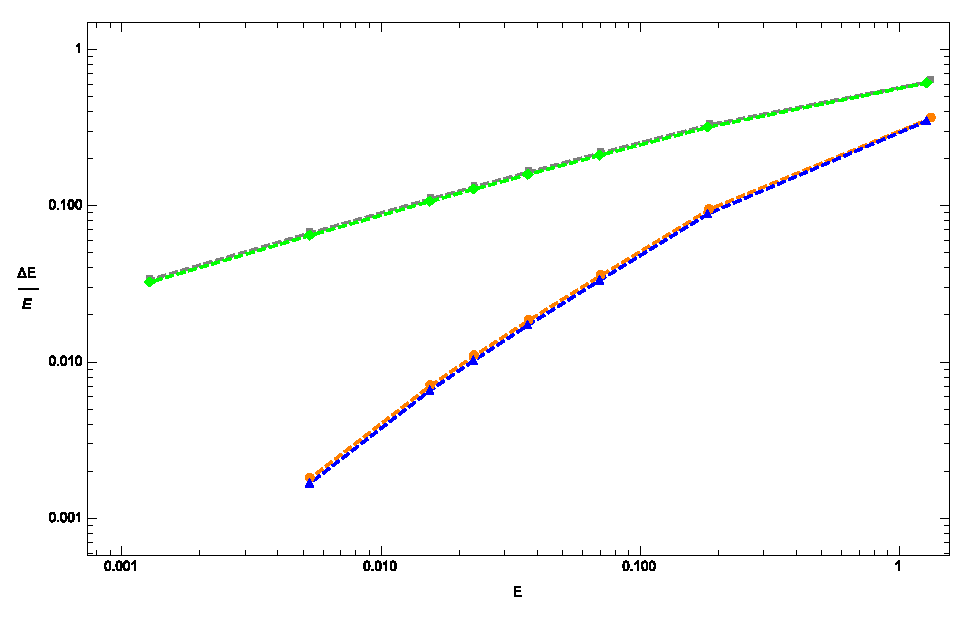
\includegraphics[width=5.2in]{Test_LepageFigure_1.eps}
  \caption{由Lepage所给能量(绿、蓝)以及拟合TrueV能量(橙、灰)得到的$E_{1n}$、$E_{2n}$ 与各自对应的真实能量的相对误差}\label{LepageFigure1}
\end{figure}
\section{\emph{Figure 2}}
在Lepage文中明确指出后两种使用有效理论的势是采用类似于真实势的解法得出束缚能级的,唯一的区别是用有效势代替真实势,另外在$Figure\;2$中也对此有明确的表述:“\emph{the nonperturbative effective theory}"。由此我并没有使用微扰论进行计算。

利用之前计算真实势束缚能的程序,我可以很容易得到有效势束缚能。

在精确到$a^2$的情况下,
\begin{equation}
  V_{eff}^{(a^2)}=-\frac{\alpha}{r}\;erf\pqty{\frac{r}{\sqrt{2}a}}+c\; a^2\;\delta_a^3(\vb{r}),
\end{equation}
精确到$a^4$的情况下,
\begin{equation}
  V_{eff}^{(a^4)}=-\frac{\alpha}{r}\;erf\pqty{\frac{r}{\sqrt{2}a}}+c\; a^2\;\delta_a^3(\vb{r})+d_1\;a^4\;\laplacian{\delta_a^3(\vb{r})}+d_2\;a^4\;\div{\delta_a^3(\vb{r})}\grad,
\end{equation}%由于有效势的系数仍需确定,这将是我所进行的第一步。
其中smeared delta functon定义为$\displaystyle\delta_a^3(\vb{r})=\frac{e^{-\frac{r^2}{2a^2}}}{(2\pi)^{\frac{3}{2}}\;a^3}$。

精确到$a^2$的有效势系数由于需要用散射相移确定,暂时不参与计算。对于精确到$a^4$的有效势,由Lepage文中给出的值,系数$c=-3.18\times4\pi$,$d_1=-0.199\times4\pi$,$d_2=0$(对S波)。
%\subsection{有效势的系数}
\subsection{S波束缚能级}
与计算真实势类似,我得到了各能级束缚能如下表:
\begin{table}[!htbp]
  \centering
  \begin{tabular}{|cccccc|}
    \hline
    % after \\: \hline or \cline{col1-col2} \cline{col3-col4} ...
    能级 & 能量计算值 & Lepage能量值 & 能级 & 能量计算值 & Lepage能量值 \\
    \hline
    1S & 1.49378 & 1.28711542 & 6S & 0.0155484 & 0.0155492598 \\
    2S & 0.182098 & 0.183325753  & \dots &   & \\
    3S & 0.0703401 & 0.0703755485 & 10S & 0.00534527 & 0.00534541931 \\
    4S & 0.0371441 & 0.0371495726 & 20S & 0.00129203 & 0.00129205010 \\
    5S & 0.022925 & 0.0229268241  &  &  &  \\
    \hline
  \end{tabular}
  \caption{$V_{eff}^{(a^4)}\;\;$S波能量对比}
\end{table}
\subsection{重复Lepage的相对误差图}
可能是由于Lepage文中所给的有效势系数精确程度不够的原因,我所重复的图中的有效势相对误差在高能级情况下并不如原文中一般快速下降,而是有停留在$10^-5$量级上的趋势。在加大之前束缚能计算精度的情况下,束缚能仅在第10个有效数字处发生改变,变化极小,因此不太可能是由于束缚能计算误差引起这种相对误差较高的情况。

相对误差如下图:
\clearpage
\begin{figure}[!htbp]
  \centering
  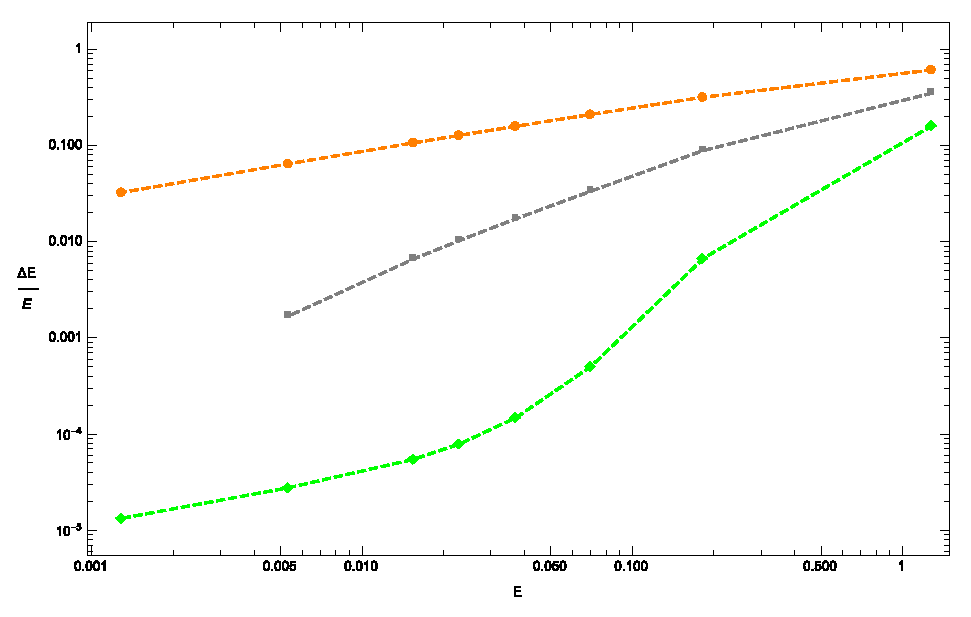
\includegraphics[width=5.2in]{Test_LepageFigure_2.eps}
  \caption{$V_1$、$V_2$、$V_{eff}^{(a^4)}$相对误差(按顺序分别为橙、灰、绿)}\label{relative error 2}
\end{figure}
由于散射相移暂时无法计算,为了验证图\ref{relative error 2}是否是由于有效势系数精度问题引起高能级数据的差别,我将系数$c$改写为$c=-(3.18+0.0008)\times4\pi$,得到下图:
\begin{figure}[!htbp]
  \centering
  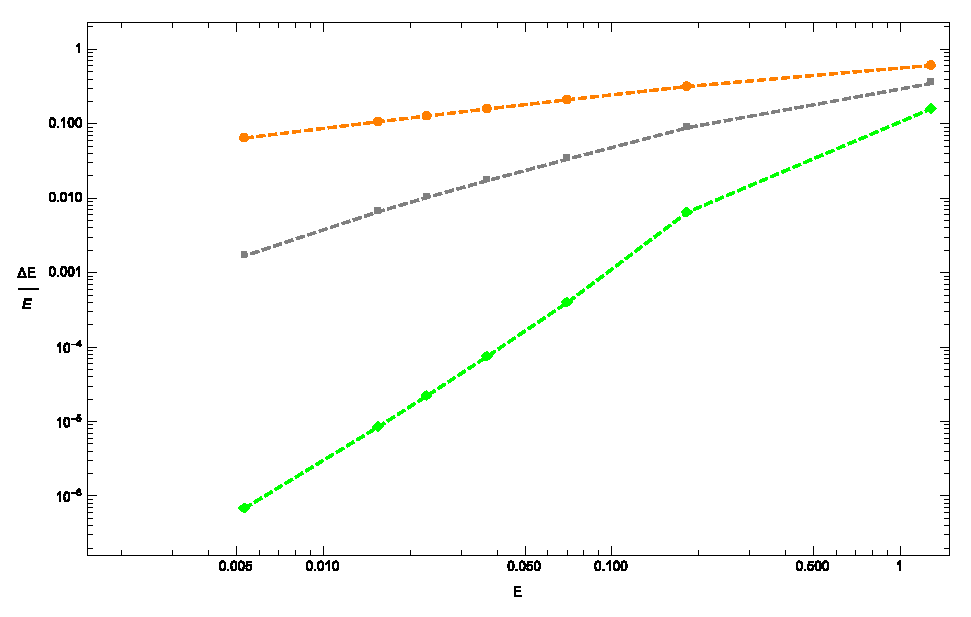
\includegraphics[width=5.2in]{Test_LepageFigure_2_2.eps}
  \caption{$V_1$、$V_2$、$V_{eff}^{(a^4)}(different\;c)$ 相对误差(按顺序分别为橙、灰、绿)}\label{relative error 2_2}
\end{figure}\\
于是可以看出图中的趋势与Lepage原图大致相同,因此可以作出猜测:数据差别的主要原因是有效势系数的精度问题。
\section{散射相移的计算尝试}
在之前的尝试中,我一直是从薛定谔方程
\begin{equation}\label{Schrodinger}
\dv[2]{r}u_l(r)+\Bqty{\frac{2m}{\hbar^2}\bqty{E-V(r)}-\frac{l(l+1)}{r^2}}u_l(r)=0
\end{equation}
入手,尝试利用边界条件
\begin{eqnarray}
% \nonumber % Remove numbering (before each equation)
  u_l(0) &=& 0 \\
  \lim_{r\to\infty}u(r) &=& \sin(kr-\frac{l\pi}{2}+\delta_l)
\end{eqnarray}
求解微分方程。由于我只需计算S波的相移,这简化了计算。但是如何在MMA中代入一个含参数的边界条件求解?
\subsection{从薛定谔方程的求解出发}
\subsubsection{对Lepage的问题求解}
只需计算S波,且已知在$r_1=50$处求解相移的话,问题就转变为:
\begin{equation}\label{Schrodinger2}
\dv[2]{r}u(r)+\frac{2m}{\hbar^2}\bqty{E-V(r)}u(r)=0
\end{equation}
\begin{eqnarray}
% \nonumber % Remove numbering (before each equation)
  \label{1}u(0) &=& 0 \\
  u(r_1) &=& \sin(kr_1+\delta_0)\label{2}
  \\  u'(r_1) &=& k\cos(kr_1+\delta_0)\label{3}
\text{  ,}
\end{eqnarray}
于是自然想到用ParametricNDSolve函数,以$\delta_0$和$E$为参数求解以上微分方程。用\eqref{Schrodinger2}、\eqref{1}及\eqref{2}\\求解出含参数的$u(r)$之后,再用FindRoot代入\eqref{3}对每一个$E$求$\delta_0$的值。

但是最终求解出的值误差极大,于是我将Lepage原文中的能量和相移以及求解出的含参数$u(r)$代入\eqref{3}中,检验方程左右两边是否相等,而其结果不等。是否有可能由于Lepage所设的势不是严格局域的,类似于Coulomb势是长程势,所以导致教科书中对相移的结论不能完全套用?Lepage在计算相移的时候是否默认$r>r1$时他的势的影响可以忽略?

%得到$\delta_0$如下表:
%\begin{table}[!htbp]
%  \centering
%  \begin{tabular}{|cccccc|}
%    \hline
%    % after \\: \hline or \cline{col1-col2} \cline{col3-col4} ...
%    能量 & 相移计算值 & Lepage相移 & 能量 & 相移计算值 & Lepage相移 \\
%    \hline
%    1S & 1.49378 & 1.28711542 & 6S & 0.0155484 & 0.0155492598 \\
%    2S & 0.182098 & 0.183325753  & \dots &   & \\
%    3S & 0.0703401 & 0.0703755485 & 10S & 0.00534527 & 0.00534541931 \\
%    4S & 0.0371441 & 0.0371495726 & 20S & 0.00129203 & 0.00129205010 \\
%    5S & 0.022925 & 0.0229268241  &  &  &  \\
%    \hline
%  \end{tabular}
%  \caption{相移}
%\end{table}
\subsubsection{验证现有程序是否可以求解S波相移问题}
由于目前的程序仅需要改变所设势$V(r)$及求解范围就可以套用到其他问题上,我先将势改为球方势阱:
\begin{equation}\label{sq}
  V(r)=
\begin{cases}
  -V_0, & \;\;\;r\leq a \\
  0, &  \;\;\;r>a
\end{cases}
\end{equation}
其解析解为:
\begin{equation}\label{s}
  \delta_0=\arctan(\frac{k \tan k_1a-k_1\tan ka}{k_1+k\tan ka \tan k_1a})
\end{equation}
其中$\displaystyle k_1=\frac{\sqrt{2m(E+V_0)}}{\hbar}$,$\displaystyle k=\frac{\sqrt{2mE}}{\hbar}$。当$l=0$,$m=1$,$\hbar=1$时,代入原程序求解,得到结果与解析解相符。

但是上述问题所涉及的相互作用势是具有明确边界的,对不具有明确边界的势来说,问题的解应该很大程度上依赖于所设的边界大小。我又设$\displaystyle V(r)=\frac{\alpha}{r^2}$,这一势在$r$较大时衰减较快,根据解析解,
\begin{equation}\label{}
  \delta_l=-\frac{\pi}{2}\bqty{\sqrt{(l+\frac{1}{2})^2+\frac{2 m \alpha}{\hbar^2}}-(l+\frac{1}{2})}
\end{equation}
当$l=0$,$m=1$,$\alpha=1$,$\hbar=1$时,$\displaystyle \delta_0=-\frac{\pi}{2}\approx-1.5707963$。由上可以看出,该相移是与能量无关的,对于任意能量相移的结果都应相同。但在将上述条件代入程序计算时发现,仅当求解范围$(0,r_1)$中$r_1$极大($r_1>1000$)时才能使结果趋近于解析解。具体解的情况见下表(最后两个相移计算时间太长,暂不列入):
\begin{table}[!htbp]
  \centering
  \begin{tabular}{|c||c|c|c|c|}
    \hline
    % after \\: \hline or \cline{col1-col2} \cline{col3-col4} ...
    \backslashbox{能量}{$r_1$} & 5 & 50 & 500 & 5000\\\hline\hline
    0.0001 & -0.03484564 & -0.3505755 & -1.4388124 & -1.5447911  \\\hline
    0.001 & -0.1122118 & -1.0148991 & -1.5267655 & -1.58000888  \\\hline
    0.01 & -0.3501234 & -1.4402778 & -1.5565288 & -1.57011187  \\\hline
    0.1 & -1.014798 & -1.5268776 & -1.56633314 &  -1.57050074 \\\hline
    1 & -1.438827 & -1.5664683 & -1.5693753 &  -1.57065489 \\
    \hline
  \end{tabular}
  \caption{不同$r_1$不同能量对应的相移计算值}\label{r^2}
\end{table}\\
当$r_1=5$时,其解明显出现问题,是否可能实际在这个边界上该势仍较大,不能近似为0,因此程序中边界条件不都成立?观察相移的值可以发现,能量和边界越小,相移值越不精确,另外能量、边界较大时微分方程的解数值上是病态的,导致未对NDSolve的求解参数进行修正时其结果精度略低。

从以上求解过程可以判断原程序在求解相移时应该是没有太大问题的(除了精度还需进一步调试),而对Lepage文中提出的相移问题进行求解时出现的偏差,可能是由于Lepage所用的真实势类似于库伦势,在$r=r_1=50$时该势仍然较大的原因,部分教科书\cite{2}中提到类似于库伦势这种非局域势不适用分波分析,而在Lepage文中也提到“\emph{These phase shifts depend
upon the radius at which they are measured because of the long Coulomb tail in
the potential $V (r)$}”,所以是否有可能Lepage所计算的相移只是利用了相移这一概念,套用相移的计算公式?还是说Lepage考虑了所谓的“\emph{long Coulomb tail}”,相对于普通的相移进行了修正?(针对前一种假设,我套用了相移公式之后,并未得到Lepage的结果。)
\subsection{积分方程求解}
求解如下积分方程:
\begin{equation}\label{Al}
  A_l(k;r)=j_l(kr)-\frac{2mik}{\hbar^2}\times\int_{0}^{\infty}j_l(kr_<)h^{(1)}_l(kr_>)V(r')A_l(k;r')r'^2\dd r'
\end{equation}
其中$r_<$($r_>$)代表$r$和$r'$中较小(较大)的一个。再将求得的$A_l(k;r)$带入到下式中:
\begin{eqnarray}
% \nonumber % Remove numbering (before each equation)
  f_l(k) &=& e^{i\delta_l}\frac{\sin \delta_l}{k} \\
   &=& -(\frac{2m}{\hbar^2})\int_{0}^{\infty}j_l(kr)A_l(k;r)V(r)r^2\dd r
\end{eqnarray}
即可求出第$l$个分波相移$\delta_l$的值。

\eqref{Al}式是一个第二类Fredholm方程,但其核(kernel function)不是非奇异的,为此我将积分下限改为$1.0\times10^{-10}$,以避过奇点。利用已有程序求解(仅有S波,即$l=0$,并设$E$(即$k$)为已知值,具体值由Lepage原文表2得到,积分上限为$r_1=50$),并代入$f_0(k)$中求解,得到$\delta_0$的值为一个复数。在对求得的$A_0$代回原式进行验证时发现,方程左右两边并不相等,说明原程序求解过程可能有问题,需要改进。

\begin{thebibliography}{b}

\bibitem{1}
Sakurai J J, Tuan S F, Commins E D. Modern Quantum Mechanics, Second Edition. Pearson Schweiz Ag, 2013.

\bibitem{2}
Griffiths, David Jeffery. Introduction to quantum mechanics. Pearson Education India, 2013.

\bibitem{3}
Lepage P. How to Renormalize the Schrodinger Equation[J]. Nuclear Theory, 1997.

\bibitem{4}
沈以淡. 积分方程[M]. 北京理工大学出版社, 1992.

\bibitem{5}
曾谨言. 量子力学(卷I)(第4版)(现代物理学丛书)(精)[M]. 科学, 2007.

\end{thebibliography}
\end{document} 